\chapter{Experimental Validation of Solution}\label{chap:results}

\section{Carefully Selecting Sample Keyframes}
Based on the chart \autoref{tab:combos} in \autoref{chap:implementation}, the general LOA combinations, concrete keyframes from the video were chosen as examples. A few keyframes in particular stood out as ones with reasonable transitions between them. It makes sense that these poses would be close in time. Three of the keyframes together make for a very short but interesting and complex clip, which is used as the baseline with which to compare the proposed method.

\section{Establishing a Baseline for Comparison}
\subsection{User Study}

\VerbatimInput{file/firstuser.txt}

The metrics recorded during the posing of characters in Rumba are: how long the program has been running since its initial launch, how many clicks the user made in the viewport for any reason, the number of posing lines drawn, and the number of selection lines drawn.

\begin{figure}[H]
	\centering
        \begin{subfigure}[b!]{0.45\textwidth}
        	\centering
                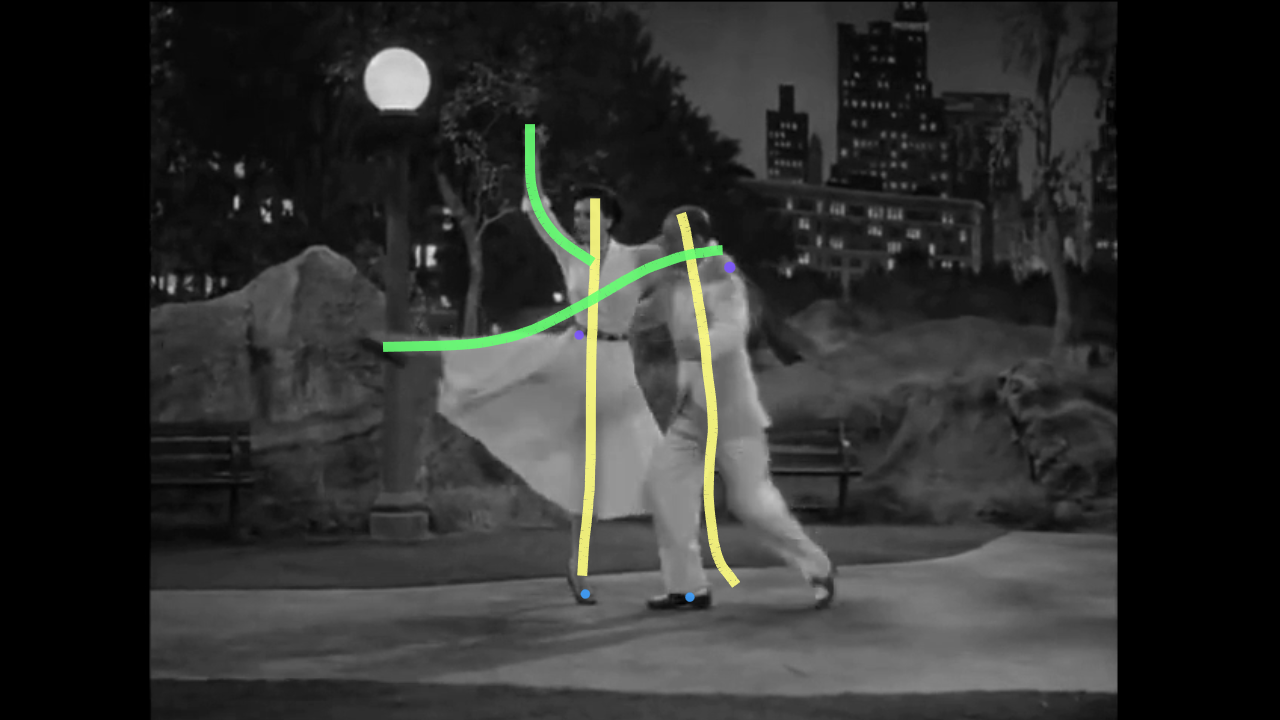
\includegraphics[width=\linewidth]{img/keyframe_case_9_(4)}
        \end{subfigure}
        \quad
        \begin{subfigure}[b!]{0.45\textwidth}
        	\centering
                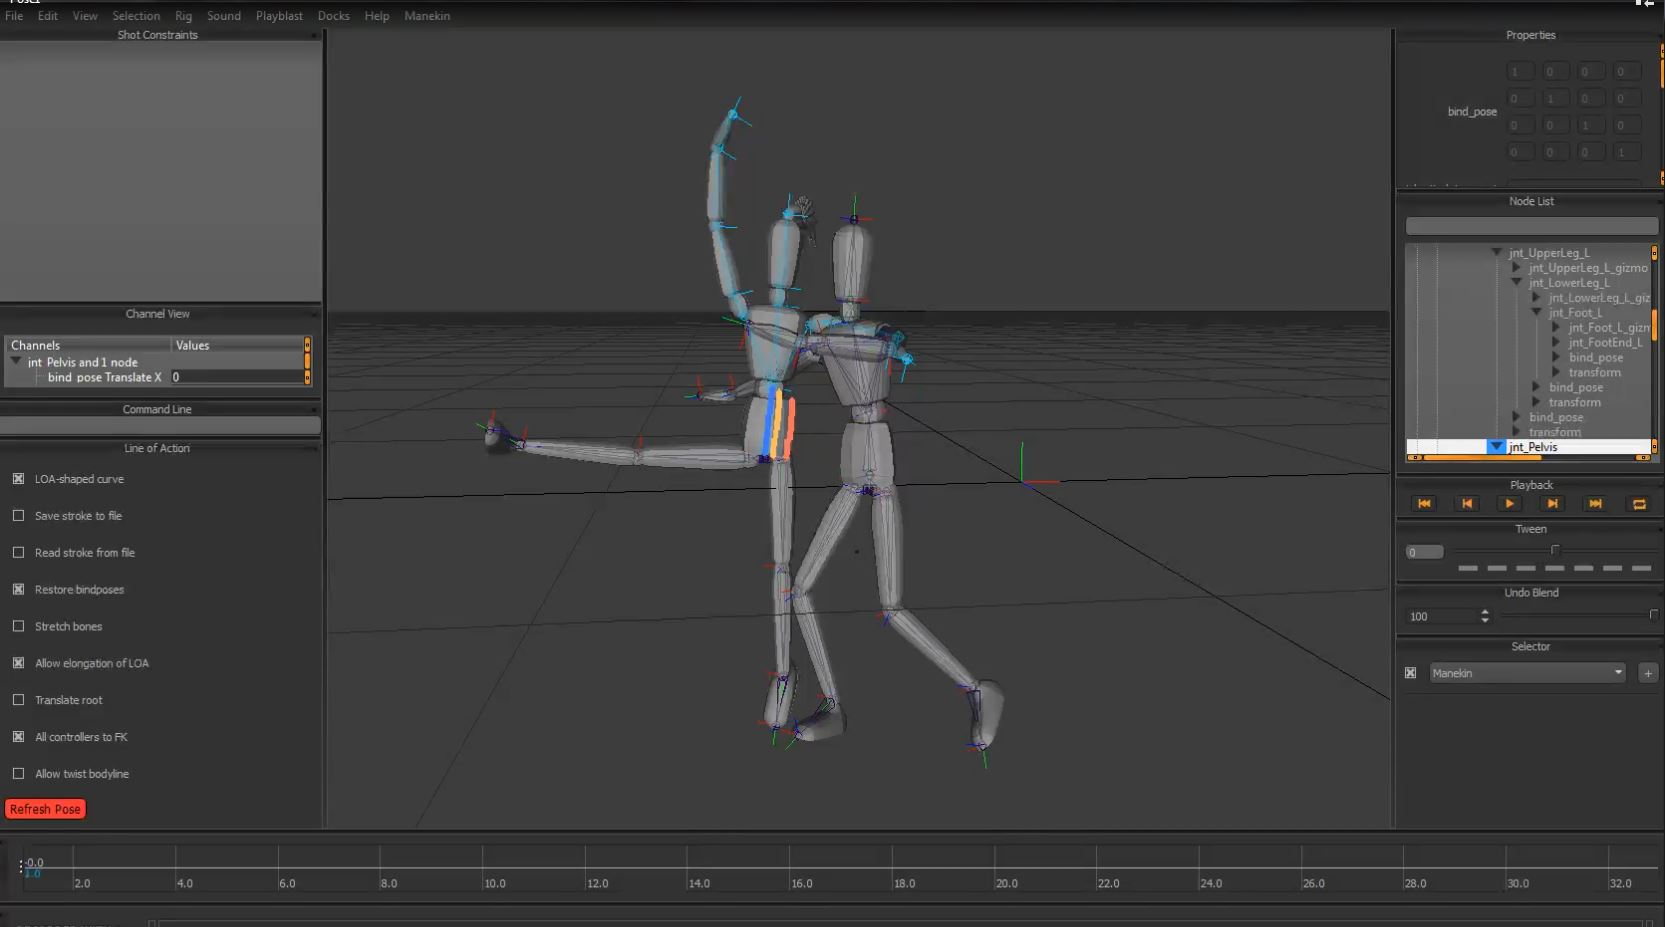
\includegraphics[width=\linewidth]{img/baselinepose1}
        \end{subfigure}%
        \caption{The first baseline pose.}
	\label{fig:bpose1}
\end{figure}

\begin{figure}[h!]
	\centering
        \begin{subfigure}[b!]{0.45\textwidth}
        	\centering
                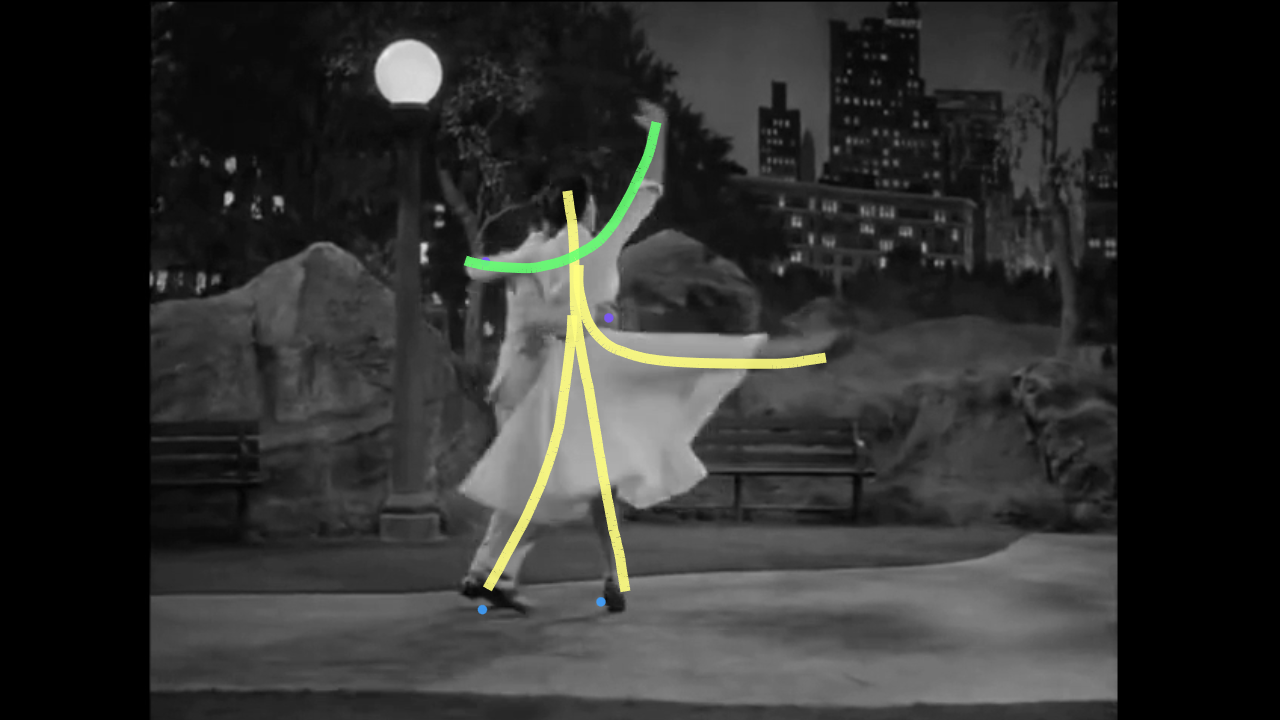
\includegraphics[width=\linewidth]{img/keyframe_case_8_(4)}
        \end{subfigure}
        \quad
        \begin{subfigure}[b!]{0.45\textwidth}
        	\centering
                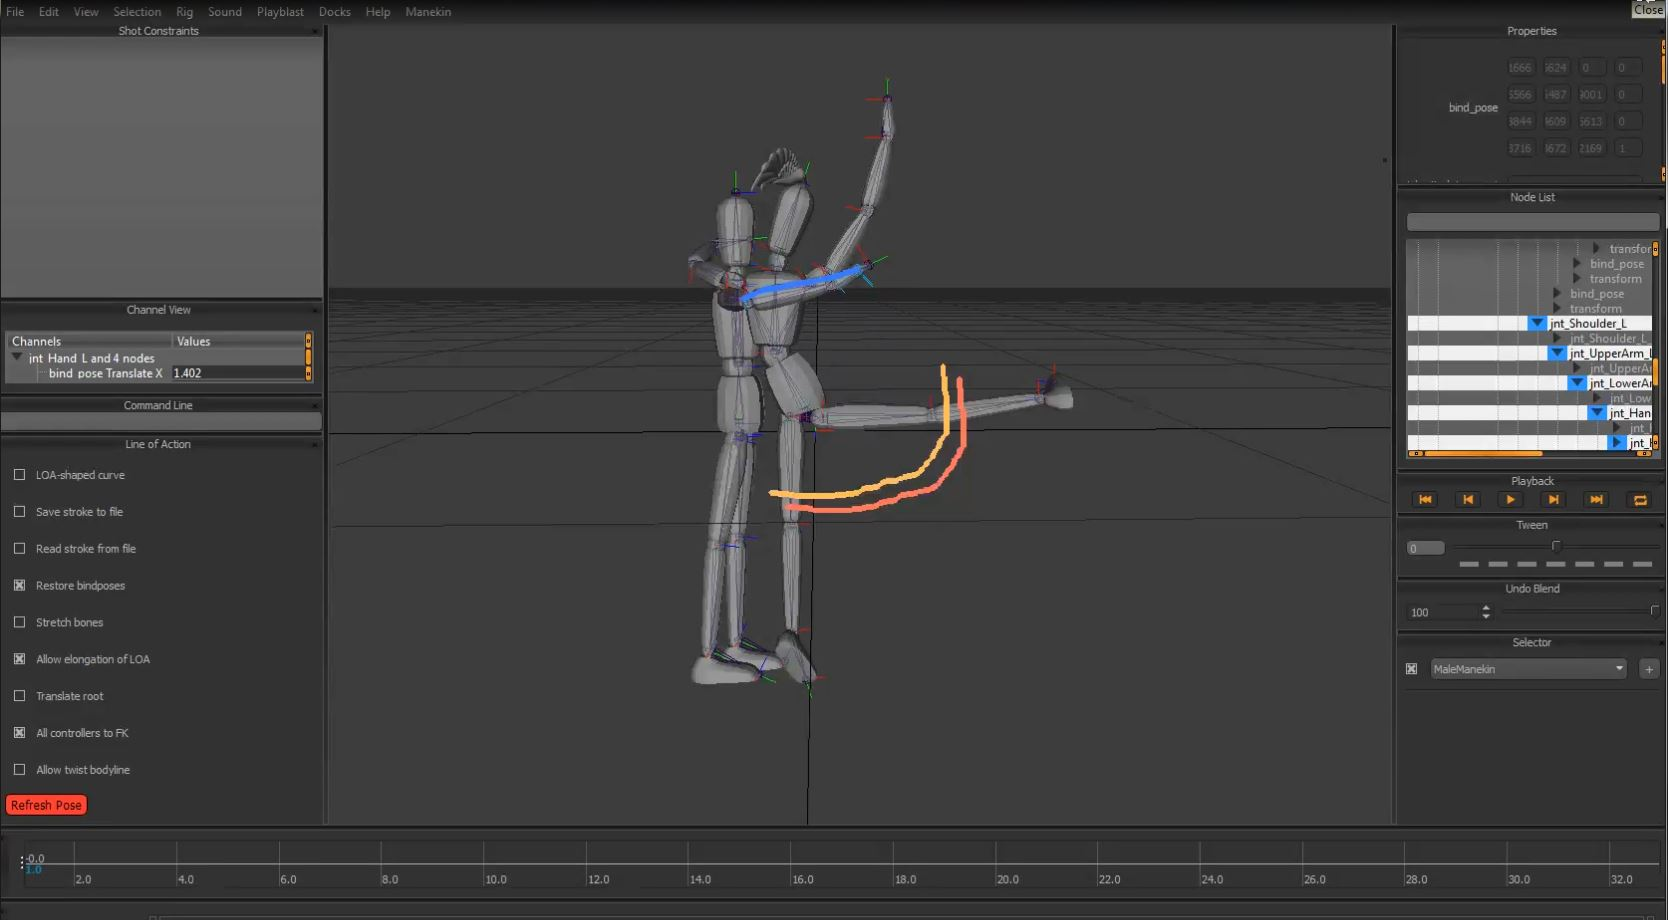
\includegraphics[width=\linewidth]{img/baselinepose2}
        \end{subfigure}%
        \caption{The second baseline pose.}
	\label{fig:bpose2}
\end{figure}

\begin{figure}[h!]
	\centering
        \begin{subfigure}[b!]{0.45\textwidth}
        	\centering
                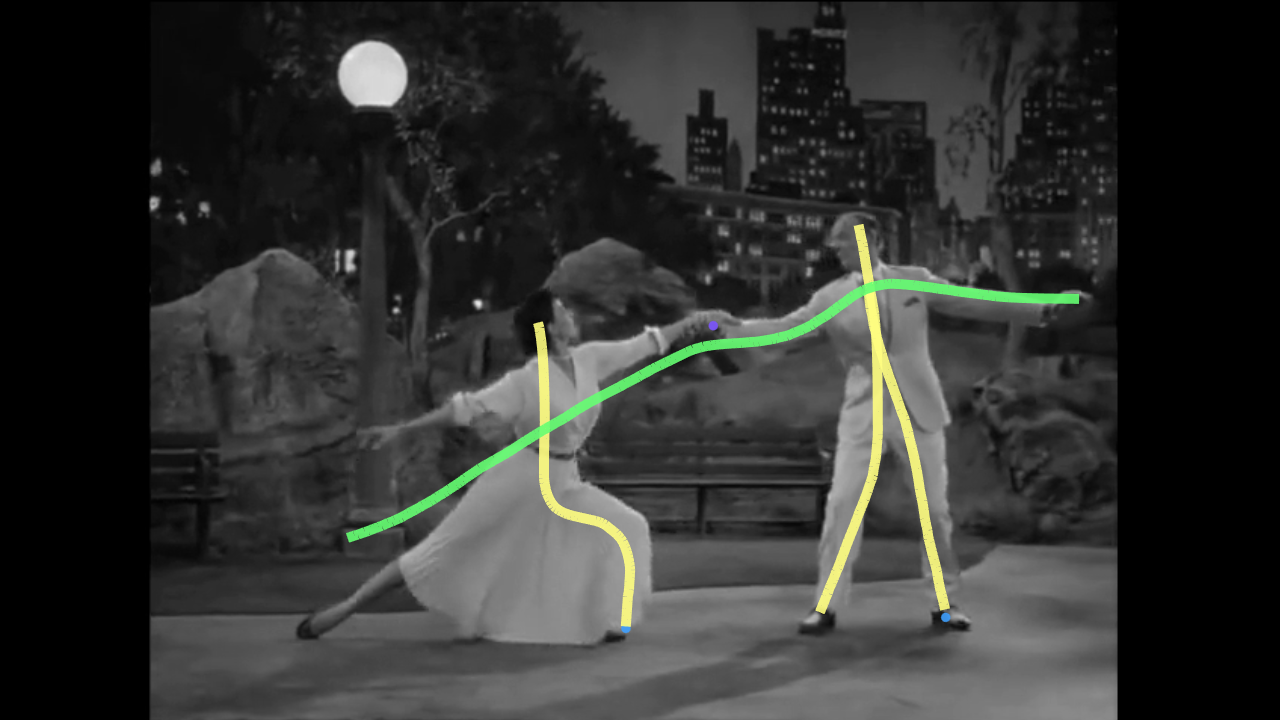
\includegraphics[width=\linewidth]{img/keyframe_case_7_(4)}
        \end{subfigure}
        \quad
        \begin{subfigure}[b!]{0.45\textwidth}
        	\centering
                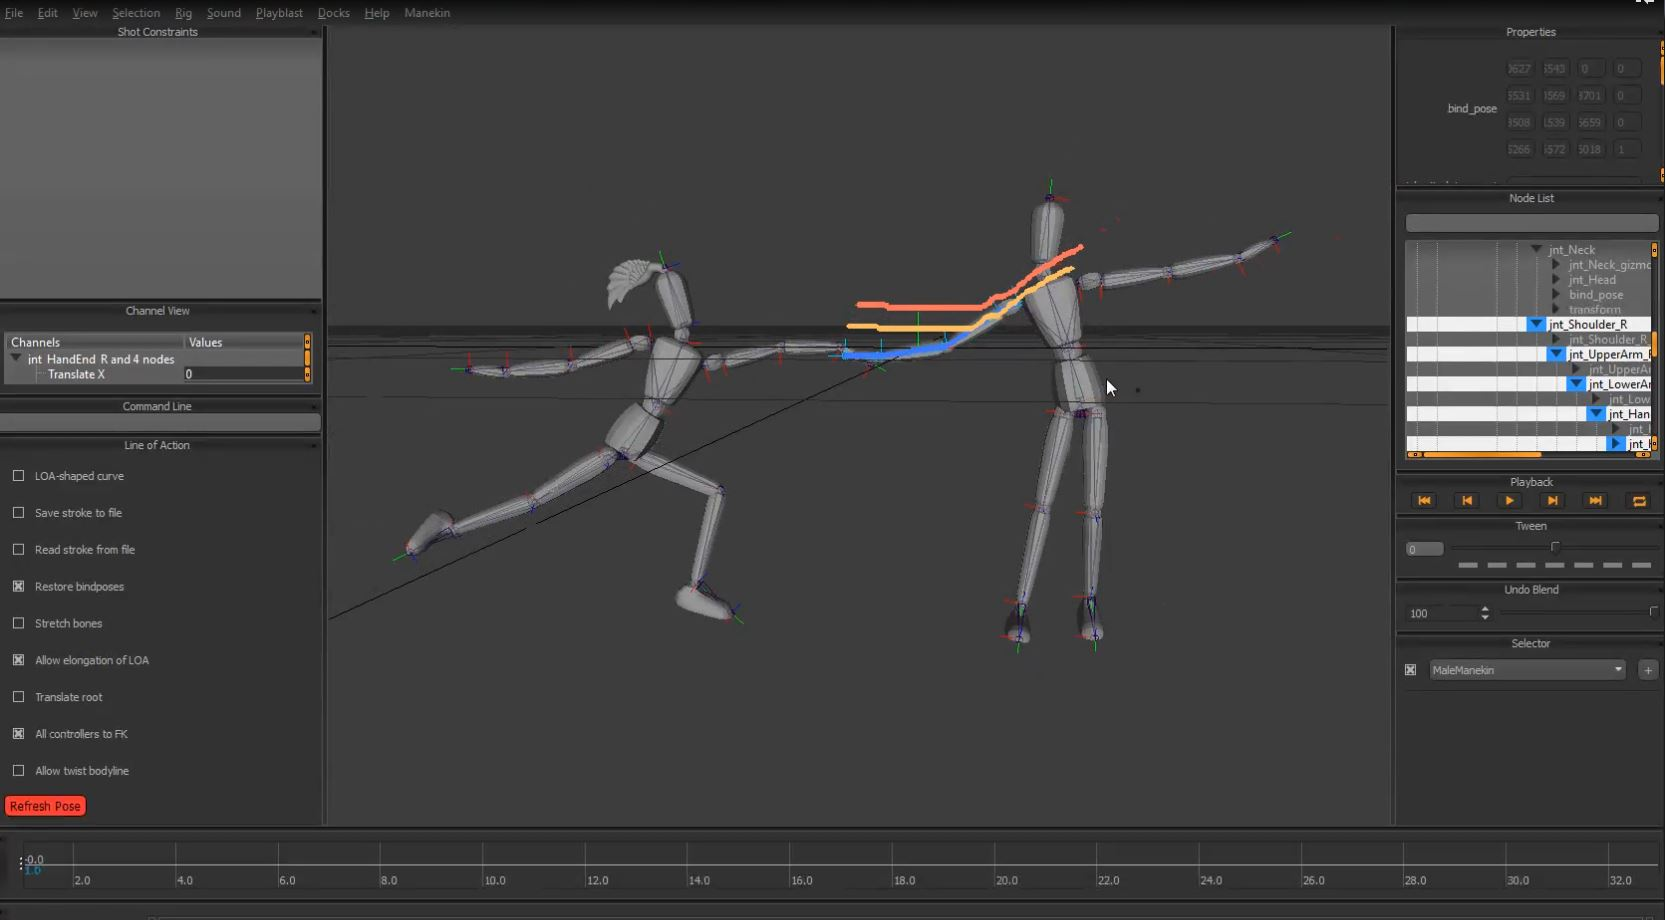
\includegraphics[width=\linewidth]{img/baselinepose3}
        \end{subfigure}%
        \caption{The third baseline pose.}
	\label{fig:bpose3}
\end{figure}

\begin{table}[h!]
\centering
\begin{tabular}{|l|l|l|l|l|}\hline
\multicolumn{5}{|c|}{Baseline User Study Results for Three Key Poses}  \\ \hline
& Total time & \begin{tabular}[c]{@{}l@{}}Number of \\ clicks in viewport\end{tabular} & \begin{tabular}[c]{@{}l@{}}Number of \\ selection lines\end{tabular} & \begin{tabular}[c]{@{}l@{}}Number of\\ posing lines\end{tabular} \\\hline
Pose 1 & \begin{tabular}[c]{@{}l@{}}11 minutes\\ 24 seconds\end{tabular} & 145                                                                     & 22                                                                   & 45                                                               \\\hline
Pose 2 & \begin{tabular}[c]{@{}l@{}}8 minutes\\ 49 seconds\end{tabular}  & 118                                                                     & 22                                                                   & 27                                                               \\\hline
Pose 3 & \begin{tabular}[c]{@{}l@{}}11 minutes\\ 59 seconds\end{tabular} & 152                                                                    & 30 & 39 \\\hline                                          
\end{tabular}
\caption{User studies for the baseline poses.}
\label{baselineresults}
\end{table}

\subsection{Experiment}
The updated user study metrics include all the metrics used in the baseline, plus the number of joints selected and the number of merges made. The same three poses made with the proposed technique are compared in accuracy to the reference photo (visually), and in efficiency and effort based on the metrics.

\VerbatimInput{file/newuser.txt}

